% =============================================================================
% Simple deck: one idea per slide, assertion titles, one chart per slide.
% Statistical detail (d, CIs, win rates per row, tables) lives in the backup.
% =============================================================================

% --- 1. Title ---
\begin{frame}[plain,noframenumbering]
\vspace*{0.4em}
\begin{columns}[T,onlytextwidth]
\begin{column}{0.68\textwidth}
\raggedright
{\color{uaibluedark}\fontsize{18}{22}\selectfont\bfseries
Geometric Filtering of LLM-Generated Samples for Few-Shot Text Classification\par}

\vspace{0.6em}
{\color{uaiorange}\rule{0.55\textwidth}{1pt}}
\vspace{0.8em}

{\large\bfseries\color{uaibluedark} Benjamín Schindler \quad Gonzalo A. Ruz}\\[4pt]
{\footnotesize\color{uaigray}
Universidad Adolfo Ibáñez, Santiago, Chile\\
Millennium Nucleus for Social Data Science (SODAS)\par}

\vspace{1.2em}
{\small\bfseries\color{uaibluedark} IEEE LACCI 2026}\\[2pt]
{\footnotesize\color{uaigray} Universidad del Pacífico \textperiodcentered{} Lima, Peru \textperiodcentered{} November 2026}
\end{column}
\begin{column}{0.30\textwidth}
\centering
\vspace{0.4em}

\includegraphics[height=1.2cm]{logos/fic.png}

\vspace{2.6em}
{\scriptsize\color{uaigray}
benjamin.schindler@alumnos.uai.cl\\
gonzalo.ruz@uai.cl\par}
\end{column}
\end{columns}
\end{frame}

% --- 2. The problem (shared with the full deck) ---
% =============================================================================
% Intro slide shared by both decks (slide 2): why few labels are a problem and
% why generated data must be reliable. Input once per document.
% =============================================================================

% Toy 2-D sketch: class A (left) vs. class B (right); the true boundary is x = 0.
\newcommand{\fewshotpanel}{%
  \draw[uaigray!50, dashed] (0,-1.15) -- (0,1.15);
  \foreach \pt in {(-1.0,0.6),(-0.7,-0.5),(-1.3,-0.1)} {\node[real] at \pt {};}
  \foreach \pt in {(0.9,0.4),(1.2,-0.6),(0.6,-0.2)} {\node[realB] at \pt {};}
}
\begin{frame}{The problem: learning from very few examples}
\small
Many real tasks have only \textbf{10--50 labeled examples per class}: labeling is slow and costly.

\vspace{0.6em}
\begin{columns}[T,onlytextwidth]
\begin{column}{0.32\textwidth}
\centering
{\bfseries\color{uaibluedark} 1.\ Few examples}\\[4pt]
\begin{tikzpicture}
  \fill[uaigraylight!60] (-1.6,-1.15) rectangle (1.6,1.15);
  \fewshotpanel
  \draw[uaiorange, thick] (-0.5,-1.15) -- (0.4,1.15);
  \draw[uaiorange, thick] (0.4,-1.15) -- (-0.55,1.15);
  \draw[uaiorange, thick] (0.15,-1.15) -- (0.2,1.15);
  \node[font=\large\bfseries, color=uaiorange, fill=uaigraylight, circle, inner sep=0.5pt] at (0.0,0.0) {?};
\end{tikzpicture}\\[4pt]
Many boundaries fit the data.\\
\textbf{Which one is right?}
\end{column}
\begin{column}{0.32\textwidth}
\centering
{\bfseries\color{uaibluedark} 2.\ Create more from them}\\[4pt]
\begin{tikzpicture}
  \fill[uaigraylight!60] (-1.6,-1.15) rectangle (1.6,1.15);
  \fewshotpanel
  \foreach \pt in {(-0.4,0.9),(-0.3,-0.2),(-1.4,0.8),(-0.9,-0.95),(-0.25,0.4)} {\node[genA] at \pt {};}
  \foreach \pt in {(0.3,0.7),(0.35,-0.8),(1.4,0.2),(0.8,0.95),(0.25,0.1)} {\node[genB] at \pt {};}
  \draw[boundary] (0.02,-1.15) -- (-0.02,1.15);
\end{tikzpicture}\\[4pt]
Reliable new examples\\
\textbf{pin the boundary down.}
\end{column}
\begin{column}{0.32\textwidth}
\centering
{\bfseries\color{uaibluedark} 3.\ But only if reliable}\\[4pt]
\begin{tikzpicture}
  \fill[uaigraylight!60] (-1.6,-1.15) rectangle (1.6,1.15);
  \fewshotpanel
  \foreach \pt in {(-0.4,0.9),(-0.3,-0.2),(-1.4,0.8)} {\node[genA] at \pt {};}
  \foreach \pt in {(1.4,0.2),(0.8,0.95)} {\node[genB] at \pt {};}
  \foreach \pt in {(0.45,-0.75),(0.55,0.1),(0.35,0.65)} {\node[genBad] at \pt {};}
  \draw[boundary=methodWorse] (1.05,-1.15) -- (0.45,1.15);
\end{tikzpicture}\\[4pt]
Wrong examples\\
\textbf{teach the wrong boundary.}
\end{column}
\end{columns}

\vspace{0.5em}
\centering
\begin{tikzpicture}
  \node[real] at (0,0) {};    \node[legendtxt] at (0.12,0) {real A};
  \node[realB] at (1.4,0) {}; \node[legendtxt] at (1.52,0) {real B};
  \node[genA] at (2.8,0) {};  \node[legendtxt] at (2.92,0) {new A};
  \node[genB] at (4.15,0) {}; \node[legendtxt] at (4.27,0) {new B};
  \node[genBad] at (5.5,0) {}; \node[legendtxt] at (5.62,0) {new ``A'' that is really B};
  \draw[uaigray!60, dashed] (9.0,0) -- (9.4,0); \node[legendtxt] at (9.45,0) {true boundary};
\end{tikzpicture}

\keymessage{We need more training data, but only data we can trust.}
\end{frame}


% --- 3. Two ways to create data ---
\begin{frame}{Two ways to create more training data}
\begin{columns}[T]
\begin{column}{0.5\textwidth}
\centering
{\large\bfseries\color{methodSMOTE} SMOTE}\\[2pt]
{\small interpolates between real examples}\\[6pt]
\begin{tikzpicture}[scale=1.0]
  \embeddingclasses
  \foreach \a/\b in {pa1/pa2, pa2/pa3, pa4/pa3, pa5/pa4, pa1/pa5} {\draw[uaiorange!70, dashed] (\a) -- (\b);}
  \foreach \a/\b/\t in {pa1/pa2/0.45, pa2/pa3/0.6, pa4/pa3/0.4, pa5/pa4/0.55, pa1/pa5/0.5} {\node[synth] at ($(\a)!\t!(\b)$) {};}
\end{tikzpicture}\\[6pt]
\good\ stays in the class \quad \bad\ vectors, not text
\end{column}
\begin{column}{0.5\textwidth}
\centering
{\large\bfseries\color{methodOurs} LLM generation}\\[2pt]
{\small writes new examples from a prompt}\\[6pt]
\begin{tikzpicture}[scale=1.0]
  \embeddingclasses
  \foreach \pt in {(-0.15,0.15),(0.25,-0.35),(-0.45,0.65),(-1.35,0.75),(-1.2,-0.85),(0.85,1.05),(2.45,0.05),(2.75,0.55)} {\node[synth] at \pt {};}
\end{tikzpicture}\\[6pt]
\good\ real, fluent text \quad \bad\ lands anywhere
\end{column}
\end{columns}

\vspace{0.4em}
\centering
\begin{tikzpicture}
  \node[real] at (0,0) {};    \node[legendtxt] at (0.12,0) {real, class A};
  \node[realB] at (2.3,0) {}; \node[legendtxt] at (2.42,0) {real, class B};
  \node[synth] at (4.6,0) {}; \node[legendtxt] at (4.72,0) {new sample for class A};
\end{tikzpicture}

\keymessage{Can we get LLM text \emph{and} SMOTE's geometric control?}
\end{frame}

% --- 3. Idea ---
\begin{frame}{Our idea: keep only the LLM samples that land near their class}
\begin{columns}[c]
\begin{column}{0.5\textwidth}
\centering
\begin{tikzpicture}[scale=1.25, every node/.append style={transform shape=false}]
  \embeddingclasses
  \draw[uaibluedark, dashed, thick] (0,0) circle (1.45);
  \foreach \pt in {(-0.15,0.1),(0.35,0.2),(-0.2,0.85),(0.7,0.65),(-0.95,0.0),(0.55,-0.75),(-0.85,-0.75),(1.15,-0.3)} {\node[kept] at \pt {};}
  \foreach \pt in {(-1.75,0.75),(-1.45,-1.25),(0.3,1.75),(2.4,0.05),(2.75,0.65),(1.75,-1.15)} {\node[rejected] at \pt {};}
\end{tikzpicture}

\vspace{0.4em}
\begin{tikzpicture}
  \node[kept] at (0,0) {};     \node[legendtxt] at (0.12,0) {kept};
  \node[rejected] at (1.5,0) {}; \node[legendtxt] at (1.62,0) {rejected};
\end{tikzpicture}
\end{column}
\begin{column}{0.5\textwidth}
\begin{enumerate}\setlength\itemsep{8pt}
  \item \textbf{Generate} 3$\times$ more samples than needed with an LLM.
  \item \textbf{Embed} them with a sentence encoder.
  \item \textbf{Keep} the ones closest to the real examples of their class.
  \item \textbf{Weight} them: closer counts more.
\end{enumerate}
\end{column}
\end{columns}

\keymessage{Question: does this beat SMOTE reliably?}
\end{frame}

% --- 4. Pipeline ---
\begin{frame}{The filter only sees embeddings, so any LLM works}
\centering
\vspace{0.4em}
\begin{tikzpicture}
  \node[stage]            (real)   at (0,0)    {\textbf{Real data}\\[1pt]{\sub 10--50 per class}};
  \node[stage]            (llm)    at (2.6,0)  {\textbf{LLM}\\[1pt]{\sub 3$\times$ surplus}};
  \node[stage]            (enc)    at (5.2,0)  {\textbf{Encoder}\\[1pt]{\sub sentence embeddings}};
  \node[stage=uaiorange]  (filt)   at (7.8,0)  {\textbf{Distance filter}\\[1pt]{\sub keep closest}};
  \node[stage=uaiorange]  (weight) at (10.4,0) {\textbf{Soft weights}\\[1pt]{\sub closer = heavier}};
  \node[stage=uaigreen]   (clf)    at (10.4,-2.2) {\textbf{Classifier}\\[1pt]{\sub e.g.\ linear SVC}};

  \begin{scope}[on background layer]
    \node[draw=uaiorange, dashed, thick, rounded corners=5pt, fit=(filt)(weight),
          inner sep=5pt, fill=uaiorange!4] (ours) {};
  \end{scope}
  \node[font=\scriptsize\bfseries, color=uaiorange, anchor=south] at (ours.north) {our contribution};

  \draw[arrow] (real) -- (llm);
  \draw[arrow] (llm) -- (enc);
  \draw[arrow] (enc) -- (filt);
  \draw[arrow] (filt) -- (weight);
  \draw[arrow] (weight) -- (clf);
  \draw[arrow] (real.south) |- node[lbl, pos=0.75, below] {real samples} (clf.west);
\end{tikzpicture}

\keymessage{No fine-tuning: just prompting, embedding and filtering.}
\end{frame}

% --- 5. Soft weighting ---
\begin{frame}{Closer samples get a larger training weight}
\begin{columns}[c]
\begin{column}{0.42\textwidth}
\large
\textbf{Score} = how close a sample is to the real examples of its class.

\vspace{0.8em}
\textbf{Weight} = score$^2$

\vspace{0.8em}
\normalsize
A half-way sample counts only \textbf{one quarter}.
\end{column}
\begin{column}{0.58\textwidth}
\centering
\begin{tikzpicture}
\begin{axis}[
  lacci, width=7.2cm, height=5.4cm,
  xmin=0, xmax=1, ymin=0, ymax=1.05,
  xtick={0,0.5,1}, ytick={0,0.5,1},
  xticklabels={far,,close}, yticklabels={0,,1},
  xmajorgrids, ymajorgrids,
  xlabel={closeness to the class (score)},
  ylabel={training weight},
  legend pos=north west, clip=false,
]
  \addplot[methodSMOTE, thick, dashed, domain=0:1, samples=2] {x};
  \addlegendentry{linear}
  \addplot[uaiorange, line width=1.8pt, domain=0:1, samples=60] {x^2};
  \addlegendentry{ours (squared)}
  \draw[uaigray, densely dotted] (axis cs:0.5,0) -- (axis cs:0.5,0.25) -- (axis cs:0,0.25);
  \fill[uaiorange] (axis cs:0.5,0.25) circle (2.2pt);
  \node[font=\small, color=uaiorange, anchor=north west] at (axis cs:0.52,0.22) {$\tfrac{1}{4}$};
\end{axis}
\end{tikzpicture}
\end{column}
\end{columns}
\end{frame}

% --- 6. Setup ---
\begin{frame}{We tested it broadly}
\vspace{0.6em}
\begin{tcbraster}[raster columns=5, raster column skip=0.22cm, raster equal height,
                  raster before skip=0pt, raster after skip=0pt]
\iconcard{\glyphdata}{13}{datasets}{uaiblue}
\iconcard{\glyphmethods}{10}{augmentation\\methods}{uaiblue}
\iconcard{\glyphclf}{5}{classifiers}{uaiblue}
\iconcard{\glyphllm}{5}{LLMs}{uaiblue}
\iconcard{\glyphgrid}{{\fontsize{20}{24}\selectfont 6,700+}}{configurations}{uaiorange}
\end{tcbraster}

\vspace{1.0em}
\centering
\chip{News} \chip{Spam} \chip{Hate speech} \chip{Emotions} \chip{Intents} \chip{NER}
\quad\chip[uaiorange]{2--150 classes}

\vspace{0.6em}
{\color{uaigray}\small
10, 25 or 50 examples per class
\quad\textcolor{uaiorange}{\textbullet}\quad macro F1
\quad\textcolor{uaiorange}{\textbullet}\quad paired $t$-tests\par}

\keymessage{Everything is compared against SMOTE.}
\end{frame}

% --- 7. Main result ---
\begin{frame}{Filtered LLM data beats SMOTE by +2.6 points}
\begin{columns}[c]
\begin{column}{0.32\textwidth}
\begin{headline}
\bignumber{$+2.61$ pp}{macro F1 vs.\ SMOTE}
\end{headline}

\vspace{0.6em}
\centering
\small
wins in \textbf{89\%} of configurations\\[2pt]
$p<0.0001$, large effect
\end{column}
\begin{column}{0.68\textwidth}
\centering
\begin{tikzpicture}
\begin{axis}[
  lacci hbar, width=6.6cm, height=5.6cm, bar width=9pt,
  xmin=-0.6, xmax=3.0, xtick={0,1,2,3},
  ymin=1, ymax=6, ytick={1,...,6},
  yticklabels={\textbf{Ours (filtered LLM)}, No augmentation, Back-translation, EDA,
               BERT contextual, T5 paraphrase},
  xlabel={$\Delta$ macro F1 vs.\ SMOTE (pp)},
  bar shift=0pt, clip=false,
]
  \addplot[fill=methodOurs, draw=none] coordinates {(2.61,1)};
  \addplot[fill=methodOther, draw=none] coordinates {(0.64,2) (-0.07,3) (-0.15,4) (-0.26,5) (-0.35,6)};
  \node[font=\small\bfseries, color=methodOurs!80!black, anchor=west] at (axis cs:2.63,1) {$+2.61$};
  \node[font=\small, color=uaigray, anchor=west] at (axis cs:0.66,2) {$+0.64$};
  \node[font=\small, color=uaigray, anchor=west] at (axis cs:0.04,3) {$-0.07$};
  \node[font=\small, color=uaigray, anchor=west] at (axis cs:0.04,4) {$-0.15$};
  \node[font=\small, color=uaigray, anchor=west] at (axis cs:0.04,5) {$-0.26$};
  \node[font=\small, color=uaigray, anchor=west] at (axis cs:0.04,6) {$-0.35$};
  \vzero[methodSMOTE, dashed, thick]
  \node[font=\scriptsize\bfseries, color=methodSMOTE, anchor=south] at (axis cs:0,0.3) {SMOTE};
\end{axis}
\end{tikzpicture}\\
{\scriptsize\color{uaigray} Selected baselines; all methods with 95\% CIs in the backup.}
\end{column}
\end{columns}

\keymessage{Newer augmentation methods do \emph{not} beat SMOTE. Filtered LLM data does.}
\end{frame}

% --- 8. t-SNE ---
\begin{frame}{The filter removes samples that land in the wrong place}
\centering
\begin{columns}[T,onlytextwidth]
\begin{column}{0.495\textwidth}
\centering
{\small\bfseries\color{uaibluedark} Before: all LLM samples}\\[2pt]
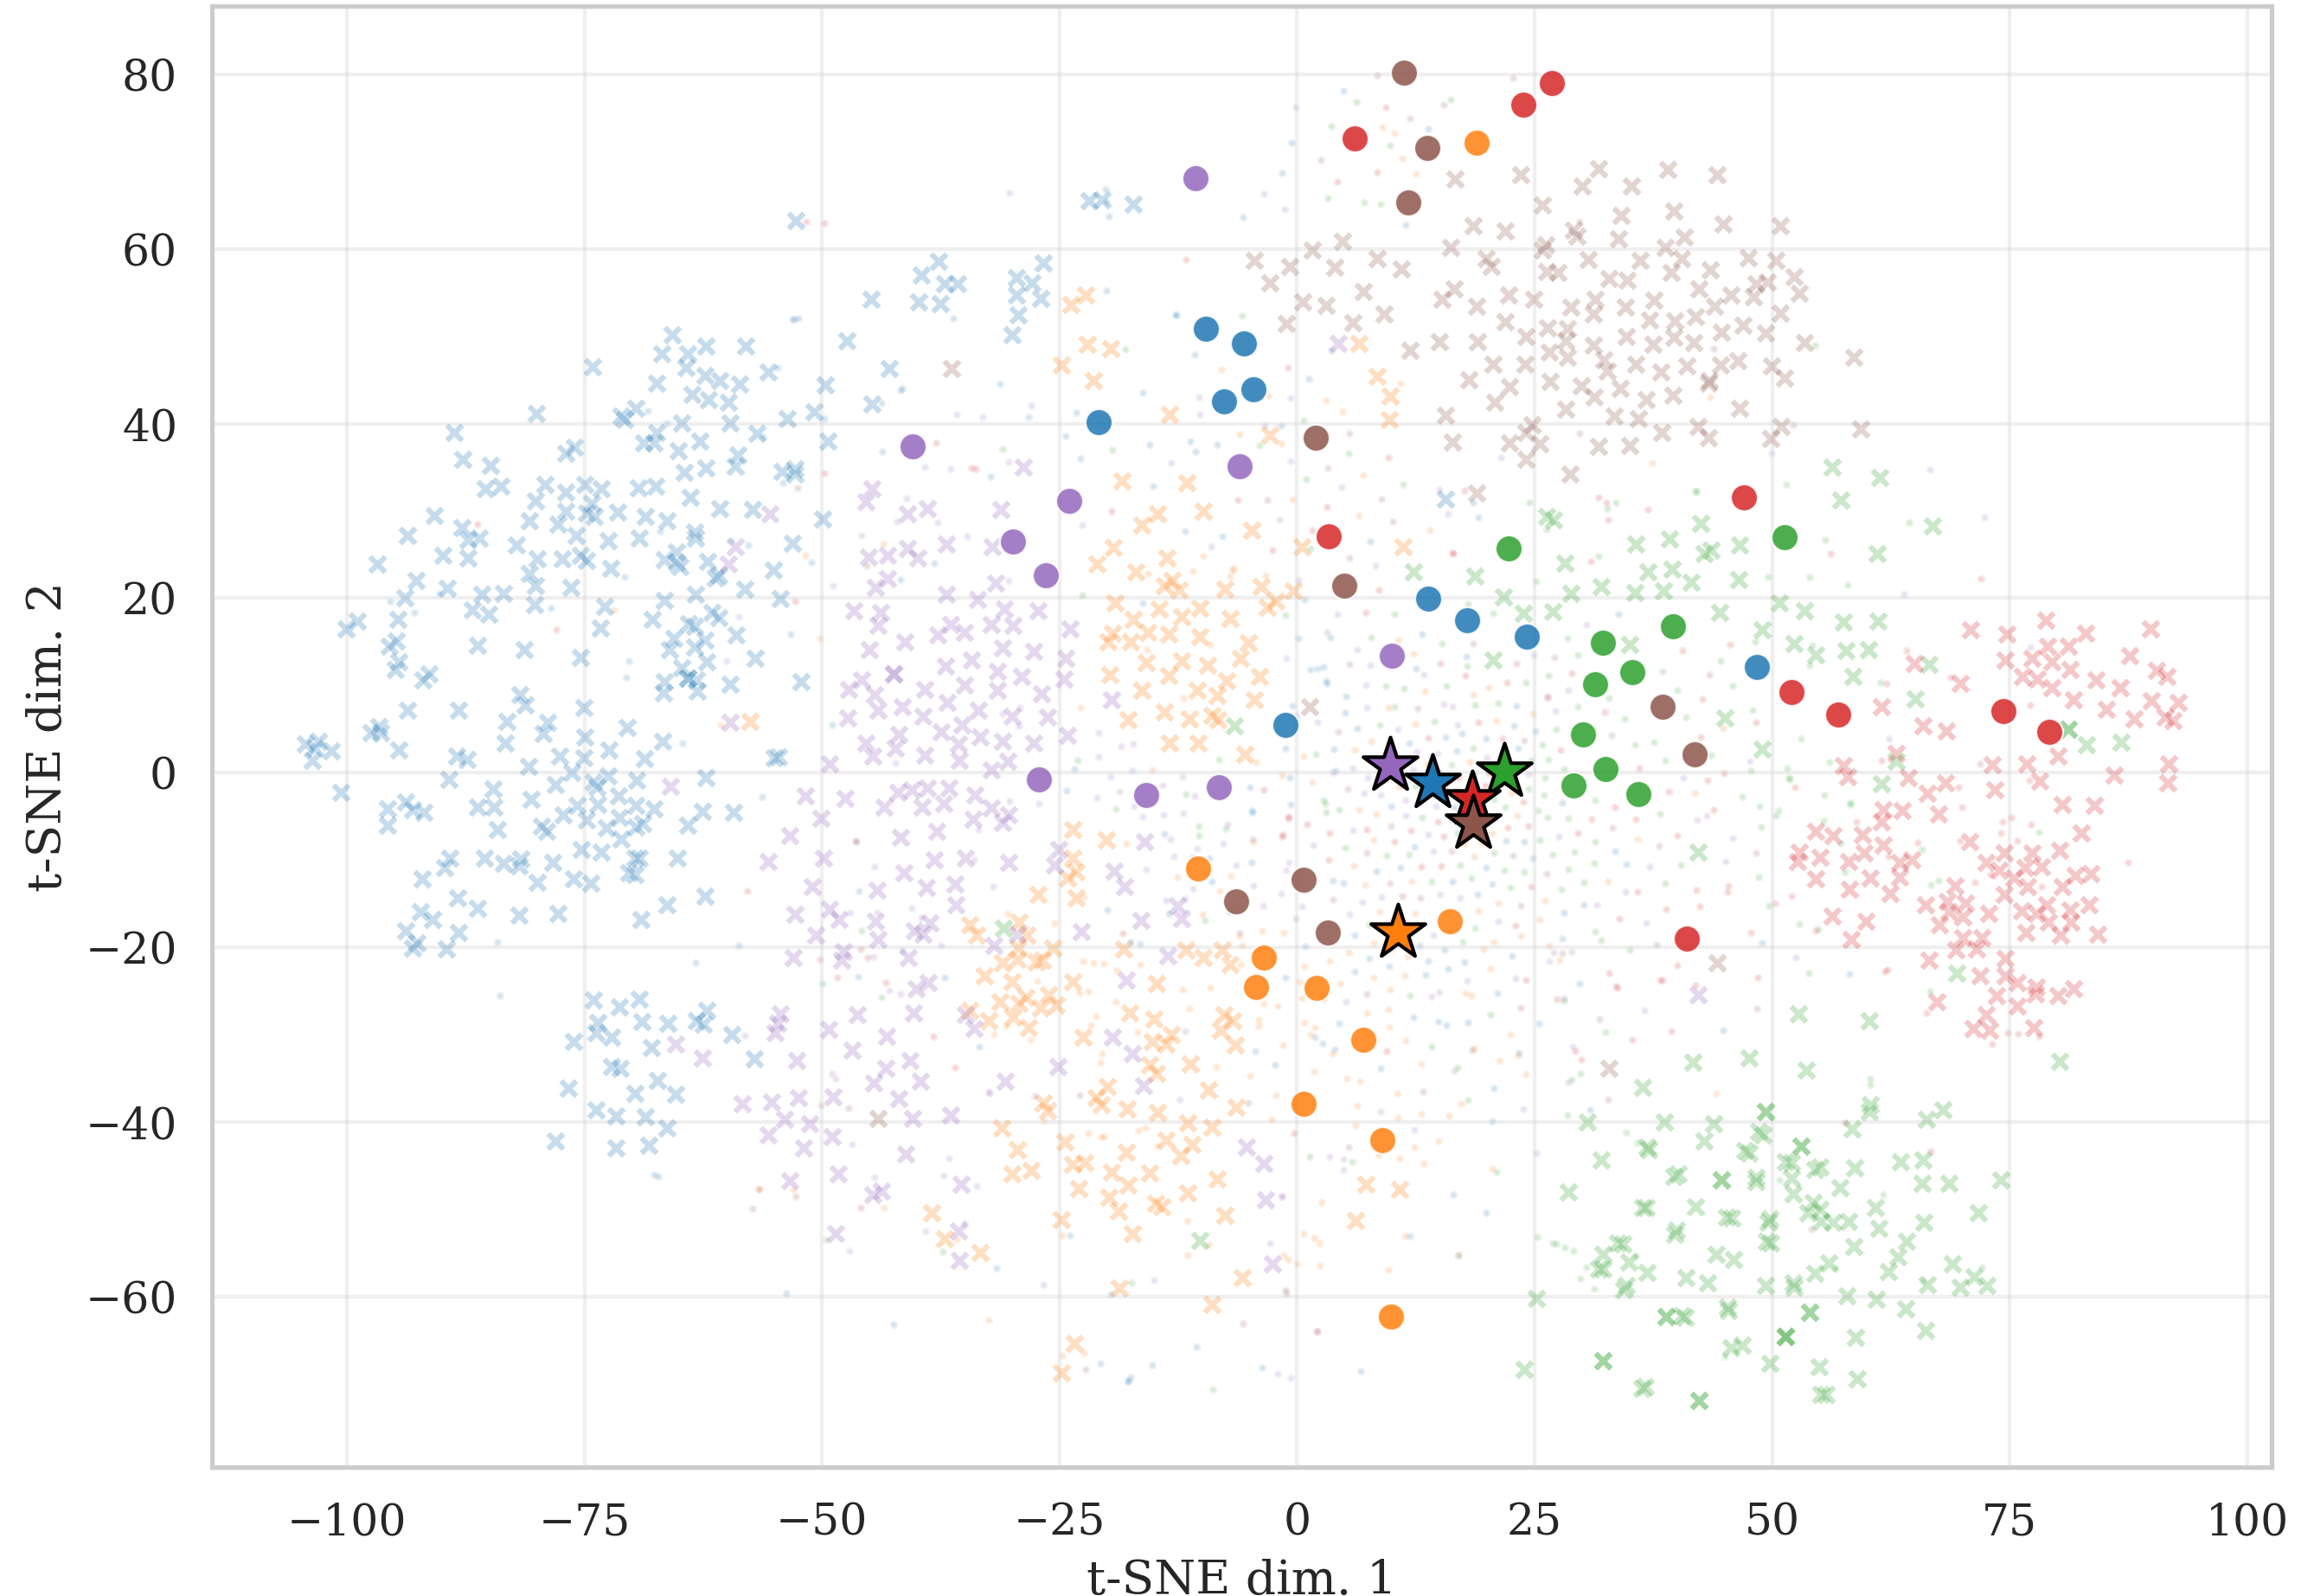
\includegraphics[width=\linewidth]{fig_tsne_emotion_before.png}
\end{column}
\begin{column}{0.495\textwidth}
\centering
{\small\bfseries\color{uaibluedark} After: kept samples}\\[2pt]
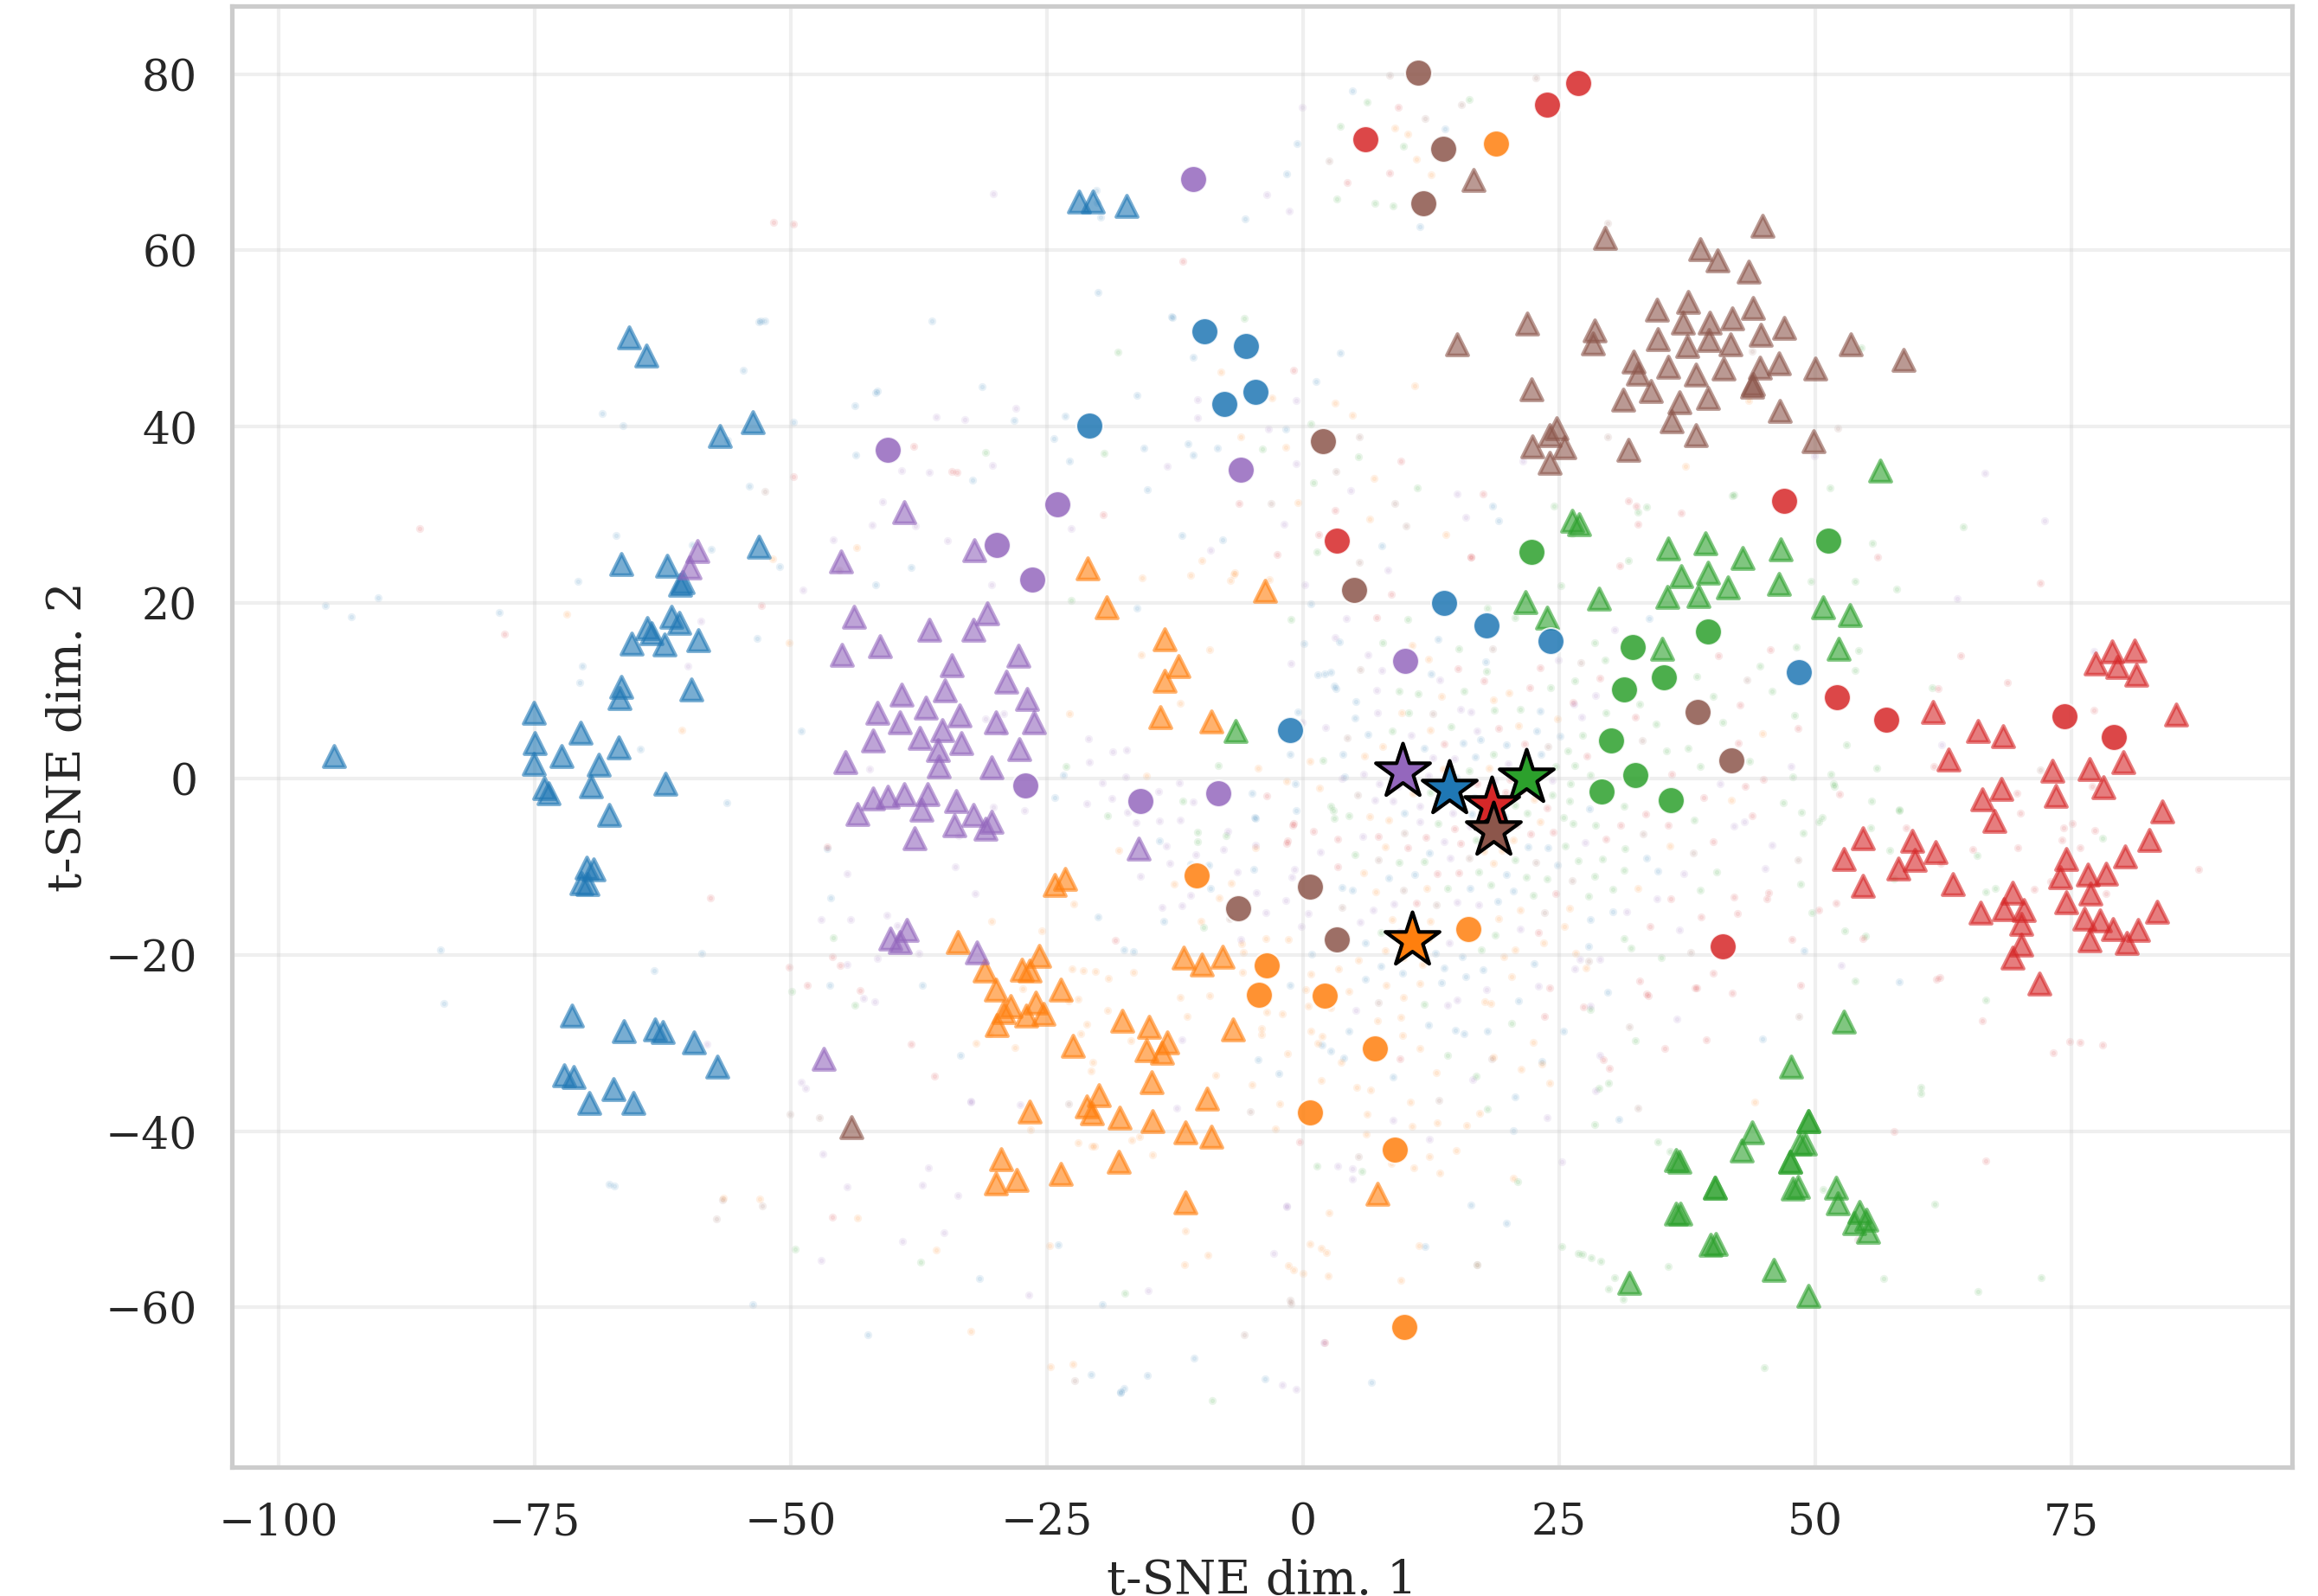
\includegraphics[width=\linewidth]{fig_tsne_emotion_after.png}
\end{column}
\end{columns}

\begin{tikzpicture}
  \foreach \c/\n [count=\i from 0] in {tabblue/anger, taborange/fear, tabgreen/joy,
                                       tabred/love, tabpurple/sadness, tabbrown/surprise} {
    \node[sw=\c] at (\i*1.3,0) {};
    \node[legendtxt] at (\i*1.3+0.1,0) {\n};
  }
  \node[legendtxt] at (8.3,0) {emotion dataset, 10 examples per class};
\end{tikzpicture}

\keymessage{Each class becomes a tighter, cleaner cluster.}
\end{frame}

% --- 9. n-shot ---
\begin{frame}{The fewer labels you have, the more it helps}
\begin{columns}[c]
\begin{column}{0.55\textwidth}
\centering
\begin{tikzpicture}
\begin{axis}[
  lacci vbar, width=7.0cm, height=5.6cm, bar width=34pt,
  ymin=0, ymax=6, ytick={0,2,4,6},
  ylabel={$\Delta$ macro F1 vs.\ SMOTE (pp)},
  symbolic x coords={10,25,50}, xtick=data, enlarge x limits=0.25,
  xticklabels={10, 25, 50}, xlabel={labeled examples per class},
  nodes near coords, nodes near coords style={font=\normalsize\bfseries, color=uaibluedark},
  nodes near coords={$+\pgfmathprintnumber{\pgfplotspointmeta}$},
]
  \addplot[fill=methodOurs, draw=none] coordinates {(10,4.89) (25,2.17) (50,0.76)};
\end{axis}
\end{tikzpicture}
\end{column}
\begin{column}{0.45\textwidth}
\large
With \textbf{10 examples} per class:\\[4pt]
macro F1 \textbf{67\% $\to$ 72\%}

\vspace{1.2em}
\normalsize
Linear classifiers gain the most\\(linear SVC: $+3.0$ pp).
\end{column}
\end{columns}
\end{frame}

% --- 10. Simple beats complex ---
\begin{frame}{Surprise: the simplest filter works best}
\vspace{0.4em}
\begin{columns}[T]
\begin{column}{0.333\textwidth}
\begin{mechbox}[colframe=uaiblue, colbacktitle=uaiblue, fontupper=\small\raggedright]{Extra metrics are redundant}
On normalized embeddings, cosine gives the \textbf{same ranking} as distance.
\end{mechbox}
\end{column}
\begin{column}{0.333\textwidth}
\begin{mechbox}[colframe=uaiamber, colbacktitle=uaiamber, fontupper=\small\raggedright]{Density needs more data}
LOF needs 20 neighbors; with 10 examples a class has only \textbf{9}.
\end{mechbox}
\end{column}
\begin{column}{0.333\textwidth}
\begin{mechbox}[colframe=uaiorange, colbacktitle=uaiorange, fontupper=\small\raggedright]{Too strict kills diversity}
Combining filters keeps only near-copies, sometimes \textbf{nothing at all}.
\end{mechbox}
\end{column}
\end{columns}

\vspace{1.0em}
\centering
\large
Distance alone beats LOF, cosine and combined filters.

\keymessage{Generate a surplus, filter lightly. More filtering is not better.}
\end{frame}

% --- 11. Robustness + NER ---
\begin{frame}{It works with any LLM, and beyond classification}
\begin{columns}[c]
\begin{column}{0.55\textwidth}
\centering
{\small\bfseries\color{uaibluedark} Gain over SMOTE by LLM (pp)}\\[2pt]
\begin{tikzpicture}
\begin{axis}[
  lacci hbar, width=6.4cm, height=4.6cm, bar width=9pt,
  xmin=0, xmax=2.7, xtick={0,1,2},
  ymin=1, ymax=5, ytick={1,...,5},
  yticklabels={Gemini 3 Flash, GPT-5-mini, Claude 4.5 Haiku, GLM-5 (open), Kimi K2.5 (open)},
  bar shift=0pt, clip=false,
  nodes near coords, nodes near coords style={font=\small, color=uaibluedark, anchor=west},
  nodes near coords={$+\pgfmathprintnumber{\pgfplotspointmeta}$},
]
  \addplot[fill=methodOurs, draw=none] coordinates {(2.31,1) (2.11,2) (1.66,3) (1.64,4) (1.49,5)};
\end{axis}
\end{tikzpicture}

{\small All 5 significant; no LLM is significantly better.}
\end{column}
\begin{column}{0.45\textwidth}
\centering
{\large\bfseries\color{uaibluedark} Named entity recognition}\\[2pt]
{\small same filter, no changes}

\vspace{0.6em}
\begin{headline}
\bignumber{$+9.26$ pp}{entity F1 vs.\ no augmentation\\wins in 9 of 9 settings}
\end{headline}
\end{column}
\end{columns}
\end{frame}

% --- 12. When / limits ---
\begin{frame}{Best for few labels and few classes}
\begin{columns}[c]
\begin{column}{0.56\textwidth}
\centering
{\small\bfseries\color{uaibluedark} Gain over SMOTE by number of classes (pp)}\\[2pt]
\begin{tikzpicture}
\begin{axis}[
  lacci vbar, width=7.6cm, height=5.0cm, bar width=13pt,
  ymin=-1.8, ymax=6.4, ytick={0,2,4,6},
  xlabel={number of classes},
  symbolic x coords={2,3,4,6,14,20,77,150}, xtick={2,3,4,6,14,20,77,150}, enlarge x limits=0.08,
  bar shift=0pt,
]
  \addplot[fill=methodOurs, draw=none]
    coordinates {(2,3.18) (3,1.86) (4,1.70) (6,5.42) (14,0.40) (20,2.36)};
  \addplot[fill=methodWorse, draw=none] coordinates {(77,-0.99)};
  \addplot[fill=methodOther, draw=none] coordinates {(150,0.01)};
  \draw[uaigray, thick] ({rel axis cs:0,0}|-{axis cs:2,0}) -- ({rel axis cs:1,0}|-{axis cs:2,0});
  \node[font=\small\bfseries, color=methodOurs!80!black, anchor=south] at (axis cs:6,5.42) {$+5.4$};
  \node[font=\small\bfseries, color=methodWorse, anchor=north] at (axis cs:77,-0.99) {$-1.0$};
\end{axis}
\end{tikzpicture}
\end{column}
\begin{column}{0.44\textwidth}
\setbeamercolor{block title}{fg=white,bg=uaigreen}
\begin{block}{Helps most}
\begin{itemize}\setlength\itemsep{2pt}
  \item 10--25 examples per class
  \item up to $\sim$20 classes
  \item the hardest classes (up to $+10$ pp)
\end{itemize}
\end{block}

\vspace{0.3em}
\setbeamercolor{block title}{fg=white,bg=uaiamber}
\begin{block}{Limits}
\begin{itemize}\setlength\itemsep{2pt}
  \item 77+ classes: no gain
  \item 50 examples per class: small gain
  \item tested in English only
\end{itemize}
\end{block}
\end{column}
\end{columns}
\end{frame}

% --- 13. Take-home ---
\begin{frame}[t]{Take-home messages}
\vspace{1.0em}
\begin{enumerate}\setlength\itemsep{12pt}\large
  \item \textbf{Filtering LLM samples by distance works:} $+2.6$ pp over SMOTE.
  \item \textbf{Keep it simple:} distance alone beats complex filters.
  \item \textbf{Plug and play:} any LLM, and it transfers to NER.
\end{enumerate}

\vfill
\begin{center}
\begin{tcolorbox}[colback=uaibluedark, colframe=uaibluedark, coltext=white,
                  width=0.8\linewidth, halign=center, arc=4pt,
                  top=2pt, bottom=2pt]
\textbf{Thank you! Questions?}\\[2pt]
{\scriptsize benjamin.schindler@alumnos.uai.cl \textperiodcentered{} gonzalo.ruz@uai.cl}
\end{tcolorbox}
\end{center}
\end{frame}
